\begin{figure}
    \centering
    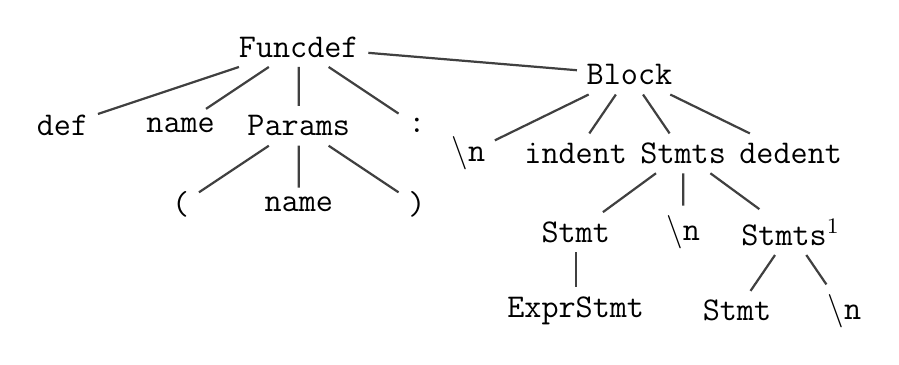
\begin{tikzpicture}
    [font=\large, edge from parent,
    % every node/.style={top color=white, bottom color=black!20,
    % ellipse, minimum size=8mm, draw=black!75,
    % thick, drop shadow, align=center},
    edge from parent/.style={draw=black!75, thick},
    level distance=1.0cm]
    \node (func) {\texttt{Funcdef}}
        child {
            node (def) {\texttt{\bfseries def}}
        }
        child {
            node (name1) {\texttt{name}}
        }
        child {
            node (params) {\texttt{Params}}
            child {
                node (openParen) {\texttt{\bfseries (}}
            }
            child {
                node (name2) {\texttt{name}}
            }
            child {
                node (closeParen) {\texttt{\bfseries )}}
            }
        }
        child {
            node (colon) {\texttt{\bfseries :}}
        }
        child [level distance=0.35cm, xscale=1.4] {
            node (block) {\texttt{Block}}
            child [level distance=1.0cm, xscale=0.65] {
                node (newline1) {\texttt{\textbackslash n}}
            }
            child [level distance=1.0cm, xscale=0.65] {
                node (indent) {\texttt{indent}}
            }
            child [level distance=1.0cm, xscale=0.65] {
                node (stmts1) {\texttt{Stmts}}
                child {
                    node (stmt1) {\texttt{Stmt}}
                    child {
                        node (expr1) {\texttt{ExprStmt}}
                    }
                }
                child {
                    node (newline2) {\texttt{\textbackslash n}}
                }
                child {
                    node (stmts2) {\texttt{Stmts$^1$}}
                    child {
                        node (stmt2) {\texttt{Stmt}}
                    }
                    child {
                        node (newline3) {\texttt{\textbackslash n}}
                    }
                }
            }
            child [level distance=1.0cm, xscale=0.65] {
                node (dedent) {\texttt{dedent}}
            }
        };
    \end{tikzpicture}
    \caption{The partial parse tree generated for \texttt{bar} in the example at
    \autoref{fig:bad-prog}}
    \label{fig:partial-parse-tree-1}
\end{figure}
